\documentclass[a4paper,12pt]{article}

%\usepackage[french]{babel}
%\usepackage[latin1]{inputenc}
\usepackage[pdftex]{graphicx}
%\usepackage{epsfig}

\def\exec{e\-xe\-cu\-tion}
\def\titre{Job-Shop Scheduling with Uncertain Durations}
\def\writers{Julien Bidot$^{1,2}$ and Philippe Laborie$^{1}$}
\def\labos{1. ILOG S.A., 9, rue de Verdun, 94253 Gentilly Cedex, France\\
           2. L.G.P./E.N.I.T., 47, av. d'Azereix - B.P. 1629, 65016 Tarbes Cedex, France}
\def\mel{\{jbidot, plaborie\}@ilog.fr}
%\def\tel{+33 (0)1 49 08 36 70}
%\def\fax{+33 (0)1 49 08 35 10}
%\def\motsclefs{}
%\def\themes{}

\title{\bfseries \titre}

\author{\writers}

%\date{\today}


\begin{document}

\bibliographystyle{alpha}

\maketitle
\vspace{-2ex}

\begin{center}
{\it \small \labos\\
\mel\\
%Tel.: \tel\\
%Fax: \fax
}
\end{center}


In this paper we present two approaches to tackle Job-Shop Scheduling Problems with temporal uncertainties. We use the constraint formalism to solve these problems.



\section{Problem description}



\subsection{Job-Shop Scheduling Problem}

A JSSP is composed of jobs. A job is a set of operations that have to be performed in a given order \textit{i.e.} there is a precedence constraint between each couple of operations in this set. Each operation is executed on a single machine. In a given job, each operation requires a different machine and the number of operations of a job is equal to the number of machines. Each machine can process one operation at a time, machines are modeled as unary resources (resource capacity of unit capacity). Operations are modeled as activities. Figure \ref{fig:jobshop} is an example of a Job-Shop Scheduling Problem. The rectangles represent the activities that have to be executed and the rectangles lengths are proportional to the processing times. The arrows represent the precedence constraints between the activities.

\begin{figure}[ht]
	\begin{center}
		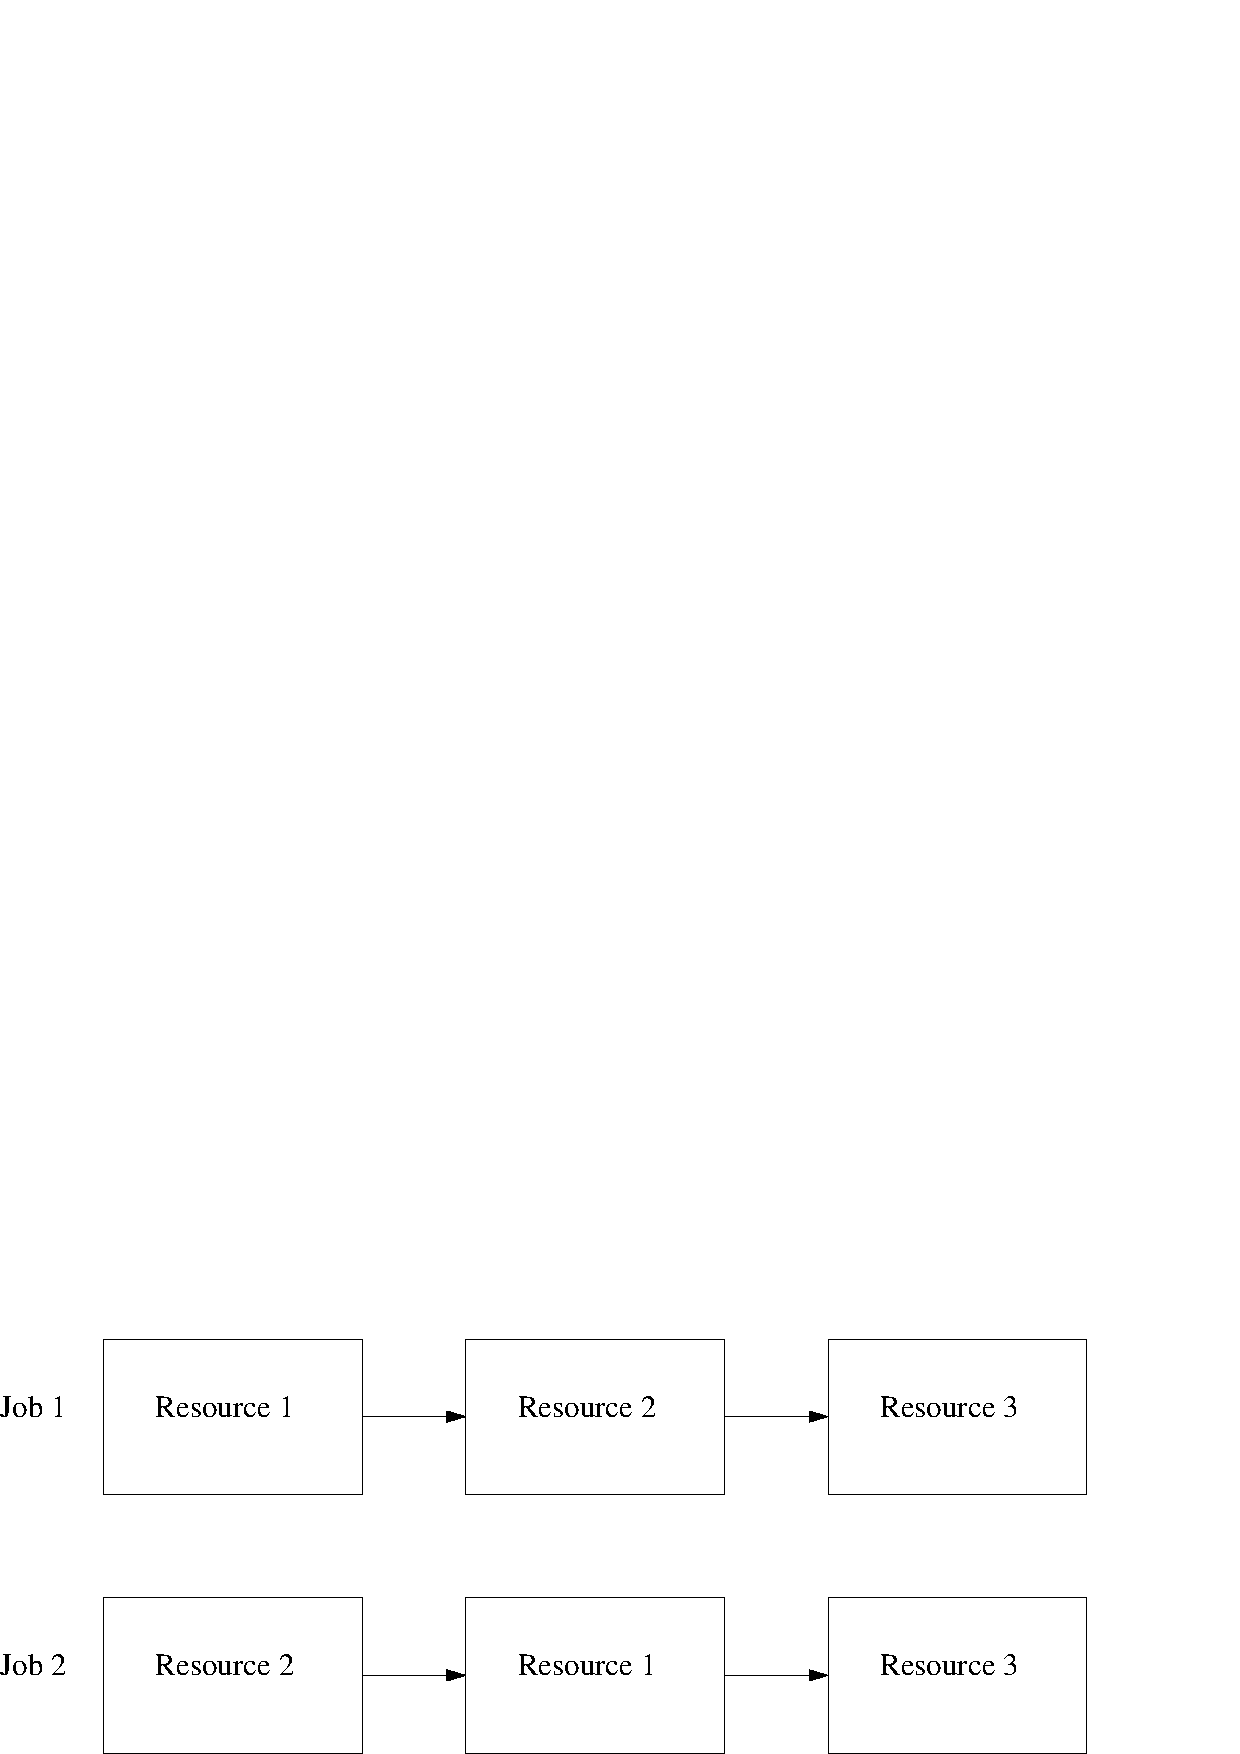
\includegraphics[width=30pc]{jobshop.pdf}
	\end{center}
	\caption{A JSSP with 3 resources and 2 jobs}
	\label{fig:jobshop}
\end{figure}


\subsection{Uncertainties}
The problem we want to solve is a Job-Shop Scheduling Problem whose activities have imprecise processing times. These processing times are modeled by variables that follow probability distributions. Each of these variables is associated with a domain. Any probability law can be used for modeling the processing time of an activity (normal, uniform, \textit{etc.}). As the processing time of an activity must be strictly positive, the laws are truncated. Figure \ref{fig:normallaw}
 depicts a normal law of average 20, standard deviation 10, truncated on the interval [0,50]. At execution, we know the effective processing time of an activity only when the activity ends and we learn this piece of information from the environment at the end time of the activity. We assume that we can get this piece of information for each activity. The only decisions are the decisions to start the activities executions. As a consequence, we know at each moment, during the execution which are the activities that have been executed, the ones that are currently executed, and the ones that have not been started yet. Suppose an activity whose processing time follows the law depicted on figure \ref{fig:normallaw} and whose execution has been started at date $t = 0$; figure \ref{fig:normallaw} displays the initial probability distribution of the end time of the activity.

\begin{figure}[ht]
	\begin{center}
		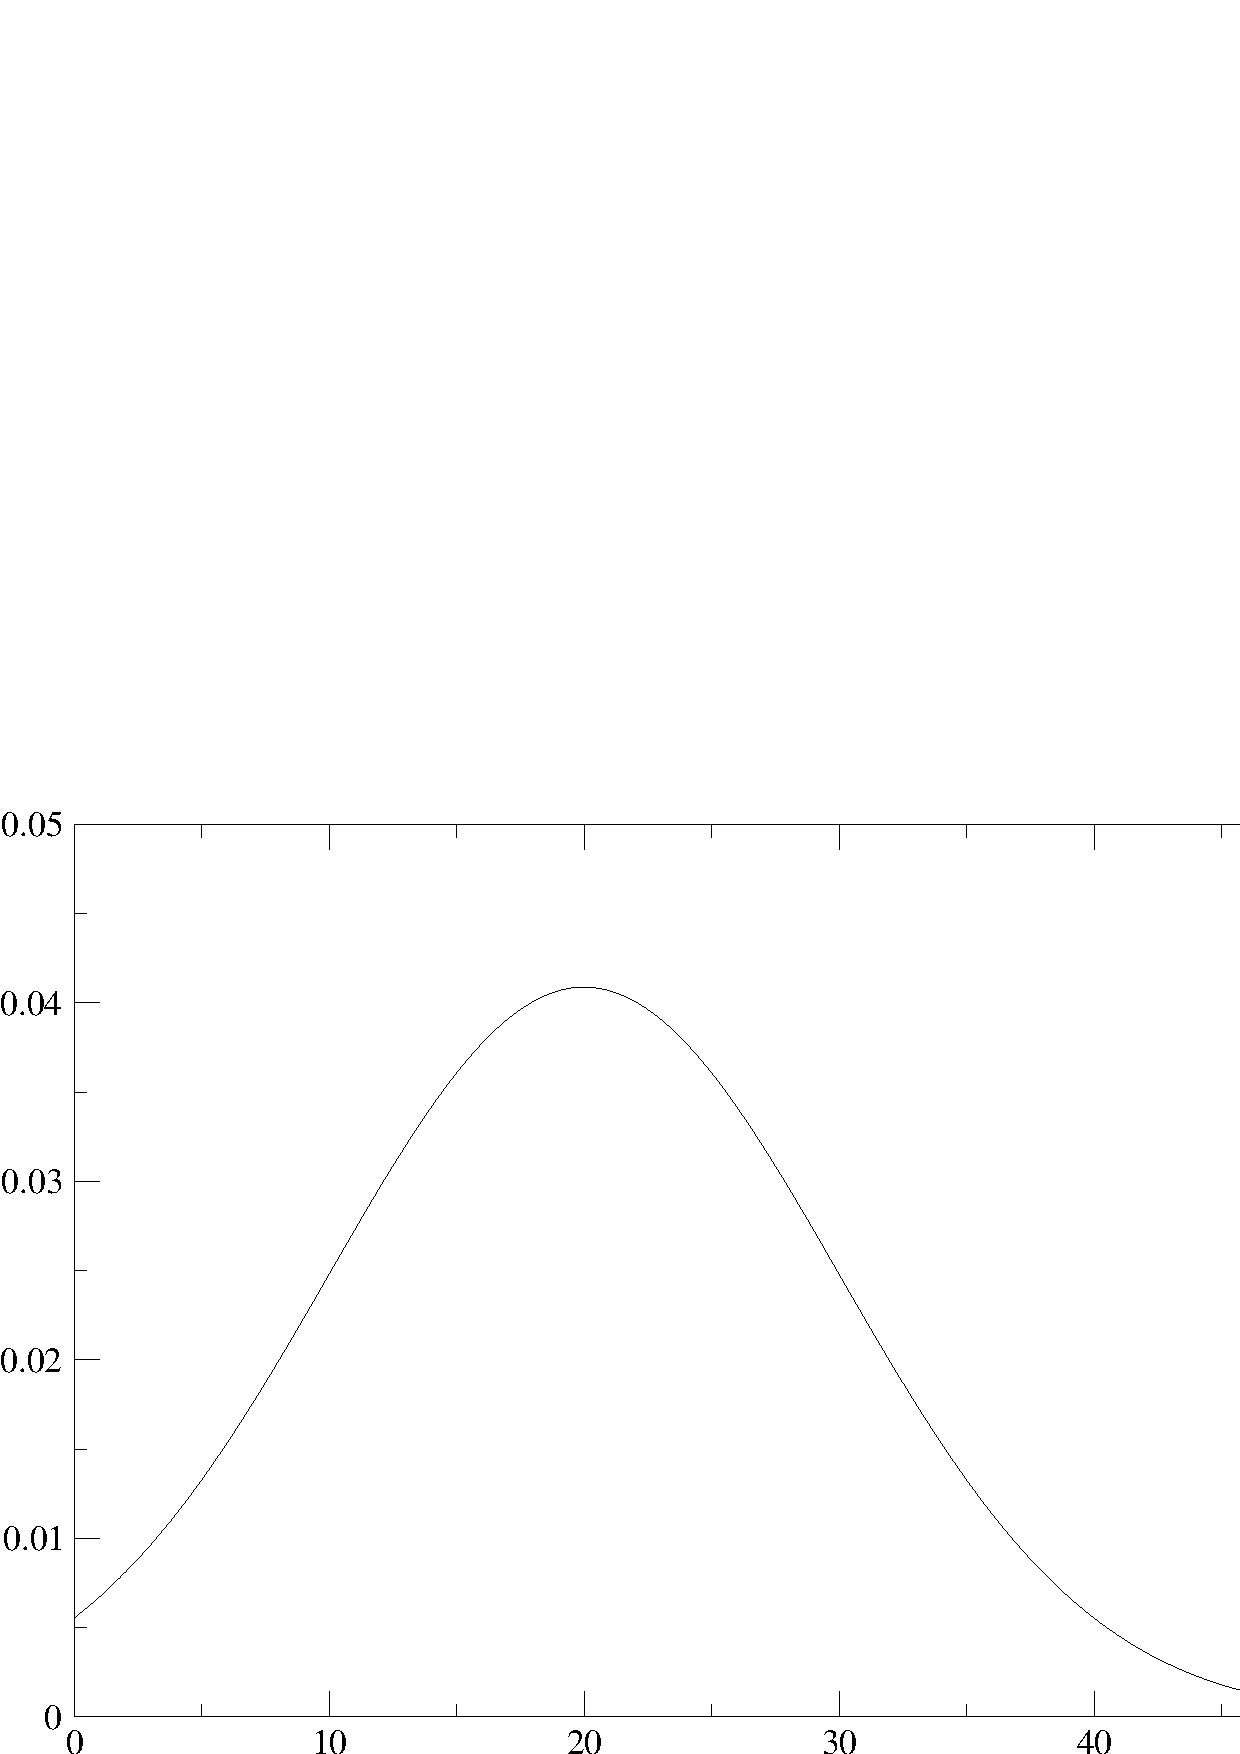
\includegraphics[width=30pc]{normallaw.pdf}
	\end{center}
	\caption{A truncated normal law}
	\label{fig:normallaw}
\end{figure}

\begin{figure}[ht]
	\begin{center}
		\includegraphics[width=30pc]{normallaw2.pdf}
	\end{center}
	\caption{A truncated normal law}
	\label{fig:normallaw2}
\end{figure}

\noindent
Now suppose that at date $t = 25$ the activity is still executing, we will assume that the probability distribution of the end of the activity is the initial law truncated on the interval [25,50] and renormalized as shown on figure \ref{fig:normallaw2}. More formally, if the initial probability law of an activity is described by a distribution function $p_0(d)$, and if the activity has been executed since $d0$ units of time, the current distribution is defined by the probability distribution $p_{d0}(d)$ as follows:\\
\begin{eqnarray}
	\forall d \in [0, d0], p_{d0}(d) = 0 \\
	\forall d>d0, p_{d0}(d) = \frac{p_0(d)}{\int_{d0}^{+\infty} p_0(t)dt}
\end{eqnarray}


\subsection{Objectives}
The main objective of this work is to try to understand if the modelization of the temporal uncertainties can bring something interesting for generating a better solution compared to the classical models. Another objective is to tune some parameters that are not yet fixed. This should also be useful because this should show us which criteria are relevant to take into account when we compare our approaches with others.



\section{Description of the two approaches}
The JSSP consists of setting the start time of each activity in order to satisfy the temporal and resource constraints and to optimize one or several criteria. One objective, which is often used, is to minimize the makespan of the JSSP \textit{i.e.} to minimize the time between the start time of the first activity executed and the end time of the last activity executed.


\subsection{Non-monotonic approach}

A first approach is to generate off-line a good "indicative schedule" (a solution schedule where all the resources are ranked), which is expected to behave well in average. One possibility would be to \emph{build such an (close to) optimal solution} corresponding to \emph{average durations} of the activities. This indicative schedule corresponds to the initial execution context. We can then either simulate this first indicative schedule or use a Bayesian network to get a first probability distribution of the makespan. We start to execute this context by following a decision policy; \emph{we could want to set the start times of the activities as soon as possible} for example. During execution the probability distributions are updated step by step as shown in subsection 1.2. This data is propagated in the constraint network associated with the current indicative schedule. This propagation can be realized in \emph{different ways}: We can either use a Bayesian network corresponding to the current indicative schedule or we can use simulation techniques. This propagation must permit to determine (and then update), among others, the probability distribution associated with the estimated makespan. \emph{One possibility} is to monitor the makespan: If the probability that the gap between the estimated makespan and the indicative makespan will get higher than a given threshold $\tau$ (for instance $\tau$ can be proportional to the makespan of the indicative schedule and has to be \textit{a priori} determined) is high enough then it means that the current schedule is slipping. In this case we will recompute a new "indicative schedule" by freezing the part that has been executed and \emph{for instance considering the average durations} of the other activities (that is, we use the same search goal as for finding the initial indicative schedule). We then get a new execution context, and the process continues.\\
There are alternatives to the makespan monitoring that is \textit{a priori} rather crude: Generally speaking we have to estimate how far the observed processing times are from those used to generate the indicative schedule. If they do not slip too much (then the makespan should not slip too much too; but this is only a consequence) then we can keep the current indicative makespan, else we must re-schedule. For example, it is possible the average makespan does not slip (because there are not many uncertainties on the critical path of the indicative schedule) while the execution of the activities that do not belong to the critical path was so that it is possible to find a much better solution after having re-scheduled. In this case it would be worth opportunistically re-scheduling when the sum of the slack times is greater than a given threshold.


\subsection{Monotonic approach}
We also investigate another approach which only performs monotonic decisions, that is, unlike the first approach, when a given decision has been taken to order activities, it cannot be questioned later on (remember that in the first approach, the indicative schedule could be recomputed from scratch). The problem with such a monotonic approach is that we must be very careful when taking a decision. From one hand we have to wait until uncertainties around the decision are low enough so that the decision is well informed. From the other hand we cannot wait too much because the schedule is executing and we do not just want to be reactive and myopic. In this approach, we have decided to solve the overall problem parts by parts during the execution. Determining when to solve a new part and how to select the part to be solved will be done thanks to information coming either from the propagation in the Bayesian network or from simulation techniques.

More precisely, suppose that we are at a given time $t$ and we are executing a schedule. We assume that part of the problem has been solved (ranked on resources) until (to simplify) a given time horizon $t_{D}$, which means that, until $t_{D}$ we could, in theory, keep on following the execution policy ("execute ASAP" for example) without making any decision. Of course, we do not want to wait until $t_{D}$ before making some decision because we would then have very few time to react and could not easily come up with a good decision (note that this certainly means that this second approach is more relevant in applications where the dynamics of the schedule is quick). From the other hand, of course, we do not want to make decisions too far in the future in regions where there is still a lot of uncertainties. Furthermore, we do not want to take the ordering decisions one by one, which would be very myopic and certainly lead to a bad makespan but rather, select a subset of activities and perform a combinatorial search on this sub-problem in order to minimize its contribution to the makespan. So there are two questions here: (1) How to design a condition that will be monitored during the execution and say "now, we can extend the current schedule by optimizing a new part of the problem" and (2) when this condition is triggered, how to select the part of the problem to be solved. For both questions, we will use information coming from the probability distributions.

(1) This condition is a mix between the fact that $t_{D}-t$ should be large enough to have time to perform a combinatorial search leading to a good solution and the fact that the minimal end times of the last activities in the part that has been solved (around $t_{D}$) should be known precisely enough. This last piece of information is given either by the Bayesian network or by a simulation technique that computes the probability distributions of these end times.

(2) When the condition above is satisfied, we still need to select an additional part of the problem to solve. We do not want to select a too big problem because: (i) We do not have an infinite time to solve it (in any case less than $t_{D}-t$) and (ii) we do not want to take decisions too far in the future as they may not be relevant. For each job we collect as sub-problem still unranked activities (with respect to resources) by chronological order (in accordance with precedence constraints) while the sum of the variances of the processing times of the selected activities (plus the variance of the end time of the last schedule activity of the job, as estimated by the Bayesian network or simulation techniques) is less than a given threshold. The sub-problem is then defined as all the collected activities on all the jobs. Once an (nearly-)optimal solution has been found to this sub-problem, this solution is added to the "solved" part of the problem and the process continues.



\section{Experimental study}


\subsection{How are instances generated?}
The instances of the JSSP with imprecise processing times are generated from classical JSSP instances. Each activity is then associated with a probability distribution defined on a domain described in section 1.2. \emph{In a first step}, each activity of processing time $p$ in the classical instance will be associated with a random processing time following a normal law of average $p$ and standard deviation $\alpha p$ with $\alpha > 0$.


\subsection{Implementation issues}

\subsubsection{Random variables}
A random variable is defined by a definition interval $[x_{min},x_{max}]$ and a probability distribution function $f$. The definition interval is uniformally discretized into $n$ steps and for each step $x_{i} = x_{min} + \frac{x_{max} - x_{min}}{n}i$ with $i\in [0,n]$, the value of the integral $F(x_i) = \int_{x_{min}}^{x_i} f(t)dt$ is stored. A reverse function $F^{-1}: [0,1] \to [x_{min},x_{max}]$, also uniformally discretized into $n$ steps is also computed by linear extrapolation.

Once this initialization has been performed, a realization of the random variable can be computed in $O(1)$ by generating a random number $y$ (uniform distribution) in $[0,1]$ and returning $F^{-1}(y)$. Note that $F^{-1}(y)$ is also computed by linear extrapolation from the discretized function $F^{-1}$.

As we have seen in section 1.2, during the execution of an activity, the probability distribution of its processing time changes because of the information that, as the activity is still executing since $x$ units of time, we know that its processing time is greater than $x$. Again, a realization of the processing time given this information can be computed in $O(1)$ by generating a random number $y$ (uniform distribution) in $[F(x),1]$ and returning $F^{-1}(y)$.

Actually for each discretized probability distribution we calculate and only store two sets of values representing respectively the integral values of this truncated law and the possible processing time values. We associate a variable with each activity that follows a uniform law. The values taken randomly by these variables represent the integral values of the corresponding truncated laws. The possible domain associated with each unform law is [0,1] (before the execution of the underlying activity). This domain is reduced during the execution of the corresponding activity and tends to be equal to 1.

\subsubsection{Histograms}
A histogram allows recording a set of realizations of a given random quantity that depends on several random variables, for instance, the makespan of the schedule or the end time of a particular activity. Histograms provide estimations of the average and standard deviation of the random quantity. We have designed a class of histogram that, by default requires $O(1)$ in memory (the realizations are not stored), the time to store a realization is in $O(1)$ and the averages and standard deviations are incrementally maintained, thus, accessing to them is also in $O(1)$. This class simply incrementally maintains $s_1=\sum_{i=1}^{n} x_i$ and $s_2=\sum_{i=1}^{n} x_i^2$ if the $x_i$ are the $n$ realizations recorded on the histogram. Then the average $avg$ is equal to $\frac{s_1}{n}$ and the standard deviation $dev$ to $\sqrt{\frac{s_2 - 2*avg*s_1 + n*avg^2}{n-1}}$.


\subsubsection{Monitoring estimated start and end times using simulation techniques}
In addition a precedence graph is generated from the constraint network: Each node represents an activity start time and each arc represents a precedence constraint between two activities (between an end time of an activity and a start time of another activity). We then sort topologically the vertices of the precedence graph and store the result in a set. Each element of the set is associated with the number of ingoing arcs and an activity start time value.


\subsection{What do we compare with? What are our criteria to compare approaches?}
To compare approaches we can use either one criterion or several criteria at the same time. One possibility is to monotore the makespan: It does not really make sense because according to the central limit theorem at the end of a chain of laws we always get a normal law; whatever value we get at the begining of the chain the estimated makespan law is not strongly affected.




\subsection{Results}

\subsubsection{Makespan monitoring}

We introduce another parameter $\sigma$ called the sensitivity factor. We reschedule when the estimated makespan $M_{est}$ is greater than the threshold, \textit{i.e.} the indicative makespan $M_{ind}$ times $\sigma$.
$M_{est} > M_{ind} \times \sigma$ is the condition that must hold for rescheduling.
We generally notice that the effective makespan is less than the first estimated makespan and the more reactive you are (lower sensitivity factor), the lower the executed makespan is but the more rescheduling.
The precision is a scale factor applied to the data.
The problem we tackle here is called la11. It is a JSSP with 20 jobs and 5 machines. The optimal makespan with the mean durations and a precision of 1000 is $1.222e^{6}$.\\

Figure \ref{fig:la11avestd} shows the estimated makespan over time. The mean and the standard deviation of the estimated makespan are represented. We monitore the makespan every 500 time steps. $\alpha$, the uncertainty factor, equals 0.3, the seed is 7 and the precision is 1000. We notice in fact that the effective end times (the green lines) correspond to the "thrusts" of the curve representing the estimated makespan (the black curve): Whenever an activity of the critical path ends the estimated makespan decreases at that time. The standard deviation (the red curve) decreases monotonically whereas the estimated makespan is not monotonic. These curves are obtained by simulating 1000 times at each step. The reschedulings (represented by the blue lines) occur during the first execution part (until about time $1e^{5}$).


\begin{figure}[ht]
	\begin{center}
		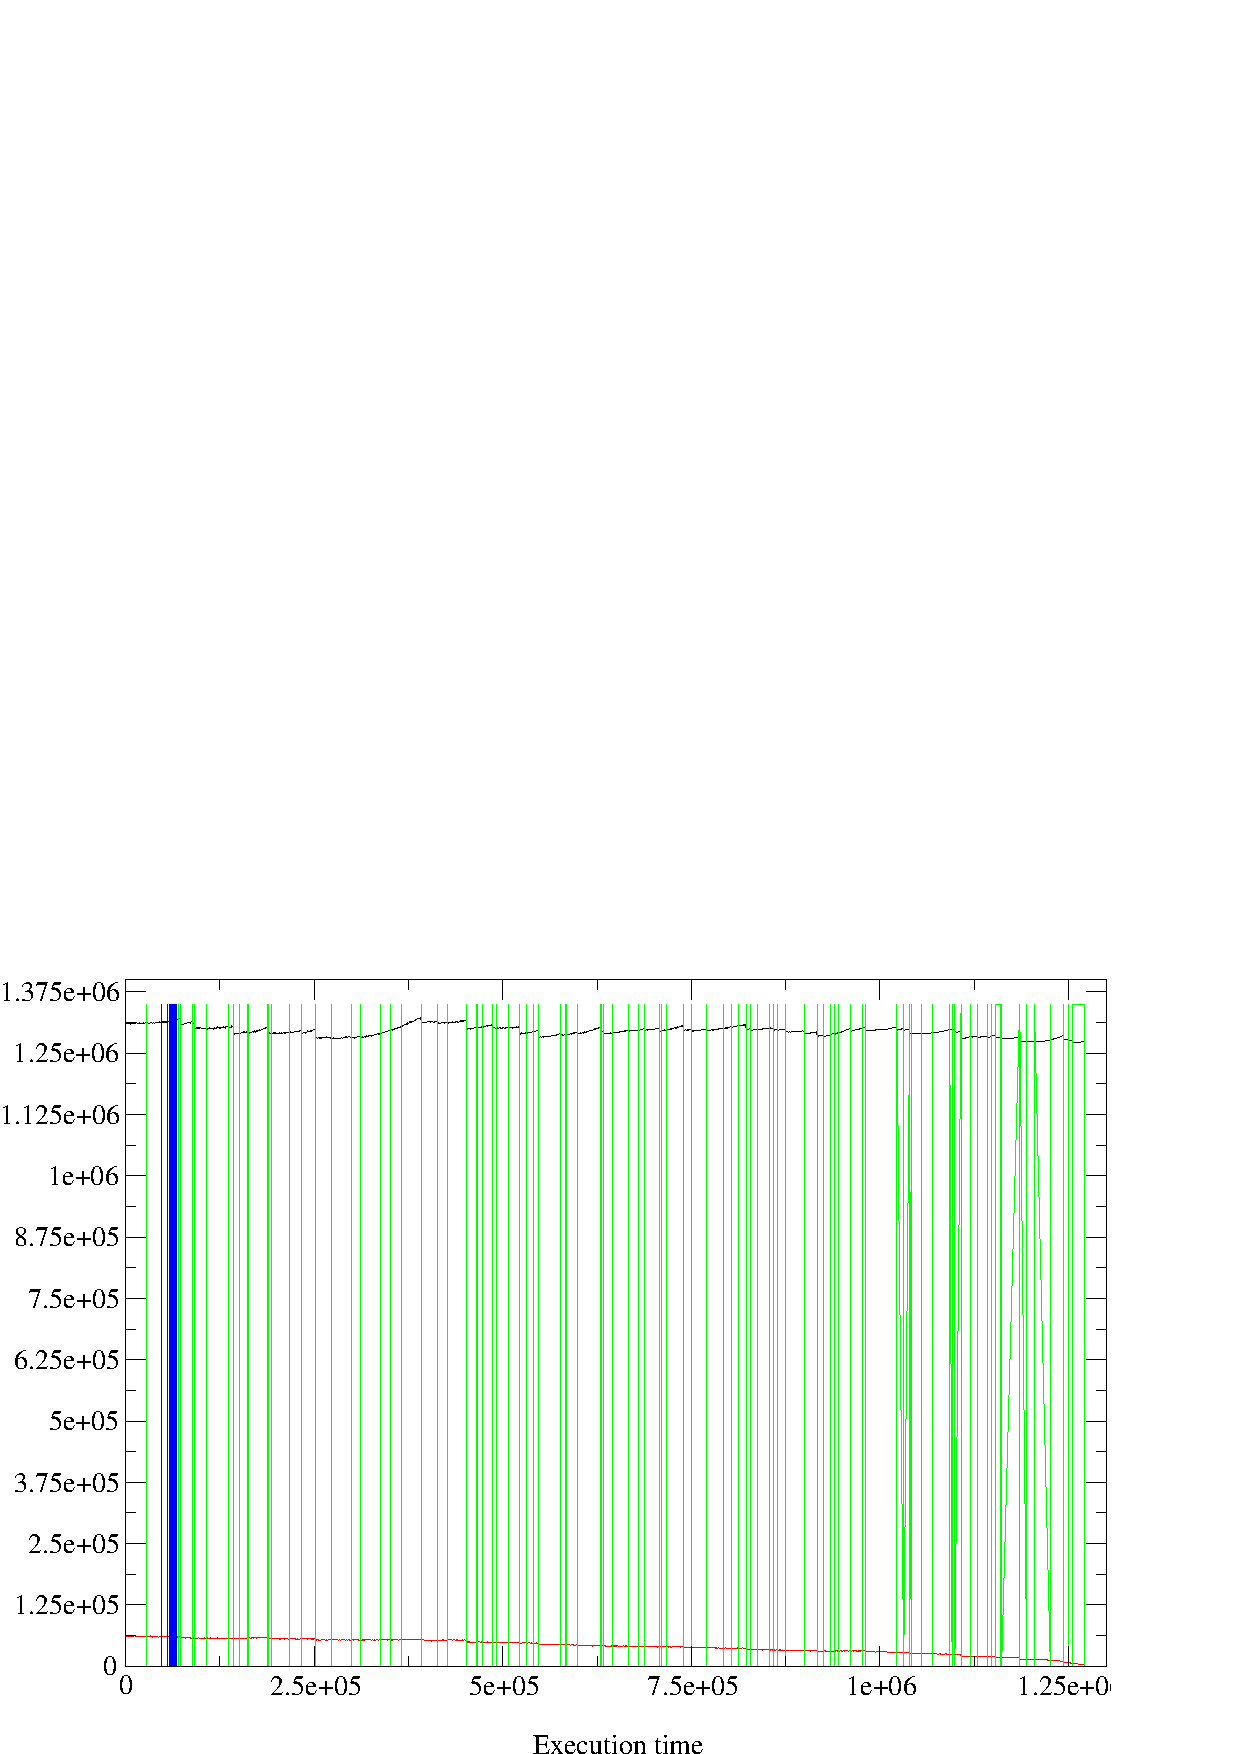
\includegraphics[width=30pc]{la11avestd.pdf}
	\end{center}
	\caption{Estimated makespan over time}
	\label{fig:la11avestd}
\end{figure}


\newpage
Figure \ref{fig:la11resched} represents the number of reschedulings according to the sensitivity factor $\sigma$. The mean and the standard deviation of the number of reschedulings are shown. We monitore the makespan when an event occurs (end or start time of an activity). $\alpha$, the uncertainty factor, equals 0.3 and the precision is 1000. These data have been obtained by simulating the schedule execution with 100 different seeds for each given sensitivity factor $\sigma$. We notice the maximum number of reschedulings is 101, \textit{i.e.} the number of activities plus one. The minimum number of reschedulings equals 0 when the sensitivity factor is too large (greater than 1.1 in this case).We also notice a quick drop for $\sigma$ between 0.98 and 1. With regard to the standard deviation we notice it is maximum and equal to 26.6 for $\sigma$ equal to 0.99 and equals 0 before 0.98 and after 1.

\begin{figure}[ht]
	\begin{center}
		\includegraphics[width=30pc]{resched.pdf}
	\end{center}
	\caption{Number of reschedulings}
	\label{fig:la11resched}
\end{figure}


\newpage
Figure \ref{fig:la11makespan} represents the mean of the effective makespan according to the sensitivity factor $\sigma$. The mean does not increase monotonically when the sensitivity factor $\sigma$ increases: We notive a quick drop between about 0.98 and 1.05.


\begin{figure}[ht]
	\begin{center}
		\includegraphics[width=30pc]{makespan.pdf}
	\end{center}
	\caption{Mean of the effective makespan}
	\label{fig:la11makespan}
\end{figure}


\newpage
Figure \ref{fig:la11makespanstd} represents the standard deviation of the effective makespan in accordance with the sensitivity factor $\sigma$. We notice a global minimum around 1.


\begin{figure}[ht]
	\begin{center}
		\includegraphics[width=30pc]{makespanstd.pdf}
	\end{center}
	\caption{Standard deviation of the effective makespan}
	\label{fig:la11makespanstd}
\end{figure}


\subsubsection{End times monitoring}






%\bibliography{article}

\end{document}